% Remplacé le 2026-11-15 par v2/papers/besoin/main.tex (version complète, erratum P1-4 compris). Conservé, non mis à jour.
\documentclass[11pt]{article}
\input{../template/preamble}
\usepackage{tikz}
\usetikzlibrary{arrows.meta,positioning,calc}
\usepackage{tabularx,enumitem}
\usepackage[most]{tcolorbox}
\newtcolorbox{encadre}[1]{colback=gray!6,colframe=gray!55,fonttitle=\bfseries,title=#1,boxrule=0.5pt,arc=1mm}
\setlist{itemsep=2pt,topsep=3pt}

\title{Estimer le besoin de soins quand on n'observe que le recours :\\
construction du module de besoin du jumeau numérique}
\author[1]{Équipe hackathon-santé}
\affil[1]{Note de travail interne, dépôt \texttt{hackathon-sante/v2}}
\date{15 novembre 2026}

\begin{document}
\maketitle

\begin{abstract}
Le jumeau numérique projette jusqu'en 2050 le nombre de sages-femmes, dentistes, pharmaciens, kinés et infirmiers du
secteur privé, du niveau de la commune jusqu'au niveau national. Il ne dit pas encore si ces effectifs \emph{suffiront}.
Pour le dire, il faut connaître le \emph{besoin} de soins de la population.

Le besoin n'est jamais observé directement. On observe le \emph{recours}, c'est-à-dire les actes remboursés. Or le
recours dépend de l'offre : on consomme moins là où les professionnels manquent, et parfois plus là où ils abondent. Le
recours seul ne permet donc pas de retrouver le besoin, ce qui oblige à faire des hypothèses.

Cette note explique ce problème sans prérequis. Elle présente ensuite cinq façons de l'aborder (M0 à M4), chacune
fondée sur une hypothèse différente, ainsi que la façon de représenter un transfert de tâches entre professions
(\enquote{et si les pharmaciens vaccinaient ?}). Elle décrit enfin les six tests, écrits et gelés avant tout calcul,
qui décideront quels estimateurs garder.

Le module est en construction. Aucun résultat chiffré du module n'est encore disponible : les nombres cités ici
décrivent les données et la littérature.
\end{abstract}
\noindent\textbf{Provenance des nombres :} \mesure{} mesuré, \derive{} dérivé, \suppose{} supposé.

\section{Pourquoi un module de besoin ?}
La question type du sujet du hackathon est : \enquote{combien de spécialistes à Clermont-Ferrand en 2035 si les
pharmaciens peuvent vacciner ?}. Elle contient en fait deux questions.
\begin{enumerate}
  \item \textbf{Combien de professionnels ?} Le jumeau y répond déjà, avec ses projections d'effectifs.
  \item \textbf{Est-ce assez ?} Pour y répondre, il faut comparer l'offre à ce dont la population a besoin.
\end{enumerate}

Aujourd'hui, la carte affiche une densité pour \num{100000} habitants. Cela revient à supposer que chaque habitant a
le même besoin. C'est faux pour deux raisons :
\begin{itemize}
  \item une personne de 85 ans a beaucoup plus besoin d'un infirmier qu'une personne de 30 ans ;
  \item une politique comme la vaccination en officine \emph{déplace} une partie du travail d'une profession vers
    une autre, sans créer un seul professionnel.
\end{itemize}

Le module de besoin calcule, pour chaque profession, territoire et année, une quantité $B$ exprimée en temps de
travail (des \enquote{équivalents temps plein}). Il en tire un \textbf{indice de couverture} :
\[
C(t) \;=\; \frac{\text{offre}(t)\,/\,\text{besoin}(t)}{\text{offre}(2026)\,/\,\text{besoin}(2026)} .
\]
$C=1$ en 2026 par construction. $C<1$ se lit \enquote{couverture moindre qu'aujourd'hui}, et $C>1$ \enquote{couverture
plus élevée qu'aujourd'hui}. On compare donc chaque territoire à lui-même, pas à une norme idéale.

\section{Besoin et recours : la difficulté centrale}

\begin{encadre}{Deux mots à ne pas confondre}
\textbf{Besoin} : la quantité de soins dont une population aurait besoin compte tenu de son état de santé (âge,
maladies, grossesses), qu'elle les obtienne ou non. C'est ce qu'on veut connaître. \emph{On ne l'observe jamais.}

\medskip
\textbf{Recours} : la quantité de soins réellement consommée, c'est-à-dire les actes remboursés par l'Assurance
maladie. C'est ce qu'on observe (Open DAMIR, patientèle des libéraux).
\end{encadre}

On peut résumer le lien entre les deux par une équation :
\[
\underbrace{R}_{\text{recours}} \;=\; \underbrace{B}_{\text{besoin}} \times
\underbrace{\varphi(A)}_{\substack{\text{part satisfaite,}\\ \text{selon l'accès } A}}
\;+\; \underbrace{D(A)}_{\text{demande induite}} .
\]
Les deux termes jouent en sens contraire.
\begin{itemize}
  \item \textbf{Là où l'offre manque}, la part satisfaite $\varphi$ est inférieure à 1. Les causes sont la distance,
    les délais ou le renoncement. Le recours est alors inférieur au besoin.
  \item \textbf{Là où l'offre abonde}, des professionnels nombreux génèrent aussi de l'activité : c'est la
    \enquote{demande induite par l'offre} \citep{evans1974}. En France, une étude sur \num{4500} médecins libéraux
    entre 1979 et 1993 la met en évidence \citep{delattre2003}.
\end{itemize}

\begin{figure}[h]
\centering
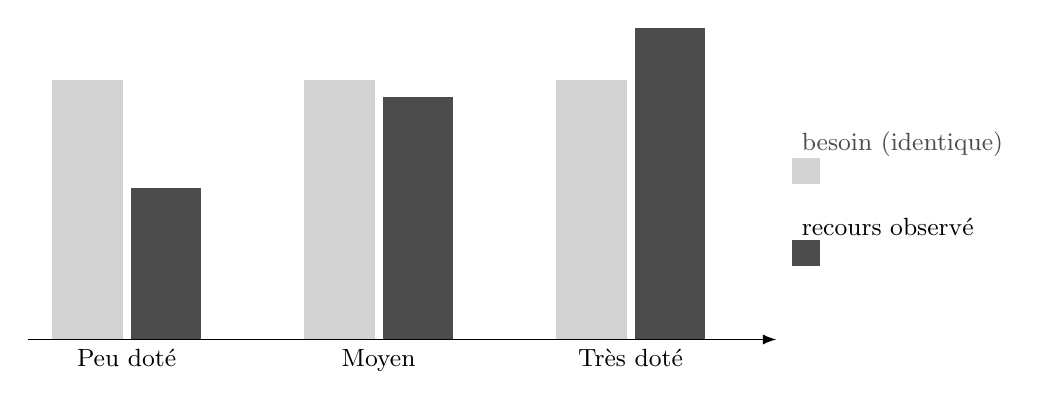
\begin{tikzpicture}[x=1cm,y=0.55cm]
  \foreach \x/\lab/\b/\r in {0/{Peu doté}/6/3.5, 3.2/{Moyen}/6/5.6, 6.4/{Très doté}/6/7.2}{
    \fill[gray!35] (\x,0) rectangle ++(0.9,\b);
    \fill[black!70] (\x+1,0) rectangle ++(0.9,\r);
    \node[below] at (\x+0.95,0) {\small \lab};
  }
  \draw[-{Latex}] (-0.3,0) -- (9.2,0);
  \node[gray!60!black,anchor=west] at (9.4,4.5) {\small besoin (identique)};
  \fill[gray!35] (9.4,3.6) rectangle ++(0.35,0.6);
  \node[anchor=west] at (9.4,2.6) {\small recours observé};
  \fill[black!70] (9.4,1.7) rectangle ++(0.35,0.6);
\end{tikzpicture}
\caption{Exemple \emph{fictif} : trois territoires avec le même besoin. Le recours observé est plus bas là où l'offre
manque, et peut dépasser le besoin là où elle abonde. Prendre le recours pour le besoin fait conclure à tort que le
territoire peu doté a moins besoin de soins.}
\label{fig:recours}
\end{figure}

\paragraph{Pourquoi on ne peut pas simplement \enquote{corriger}.}
On observe seulement le produit $B \times \varphi(A)$, plus $D(A)$. Un territoire avec un grand besoin mal satisfait
et un territoire avec un petit besoin bien satisfait peuvent donner exactement le même recours. Mathématiquement, si
l'on multiplie $B$ par n'importe quel facteur $h$ et que l'on divise $\varphi$ par ce même facteur, rien ne change dans
les données.

On dit que le besoin n'est pas \emph{identifié} à partir du recours seul. Il faut ajouter une hypothèse, et c'est là
que les estimateurs diffèrent : chacun fait la sienne, et on teste celles qu'on peut tester.

\paragraph{Une bonne nouvelle : l'indexation à 2026.}
Supposons que l'écart entre recours et besoin soit constant dans un territoire, par exemple parce que le recours y est
toujours 10~\%\suppose{} en dessous du besoin. Cet écart s'annule dans le rapport $C(2035)/C(2026)$. Seul pose problème
l'écart qui \emph{change avec le temps}, par exemple quand l'offre baisse.

On peut donc comparer 2035 à aujourd'hui dans un même territoire avec un estimateur simple. Comparer deux territoires
entre eux demande davantage.

\section{Cinq façons d'estimer le besoin}
On construit plusieurs \emph{estimateurs}, chacun avec une hypothèse déclarée. Le projet compare toujours plusieurs
algorithmes plutôt que de présenter un seul chiffre. Tous passent par la même interface de code et produisent le même
indice $C$.

\begin{table}[h]
\centering\small
\begin{tabularx}{\linewidth}{@{}l X X X@{}}
\toprule
& \textbf{Idée} & \textbf{Hypothèse qui le rend possible} & \textbf{Test qui peut l'abandonner} \\
\midrule
M0 & besoin $\propto$ population & le besoin par habitant est le même partout & référence à battre \\
M1 & population par âge $\times$ consommation de cet âge & le besoin par âge est le recours national moyen par âge & P-B1, P-B5 \\
M2a & recours \enquote{à accès moyen} & on peut neutraliser l'offre en la fixant à sa moyenne & (méthode établie) \\
M2b & recours là où il sature & au-delà d'un certain niveau d'offre, le recours plafonne & P-B2 \\
M3 & prévalence des maladies $\times$ actes par patient & une norme externe définit le besoin & P-B3 \\
M4 & accès dans l'espace (méthode de l'APL) & ne définit pas le besoin : il prend celui de M1, M2 ou M3 & P-B4 \\
\bottomrule
\end{tabularx}
\caption{Les estimateurs du module de besoin.}
\end{table}

\subsection*{M0 : proportionnel à la population}
Le besoin vaut la population multipliée par un taux unique par profession. C'est la densité pour \num{100000}
habitants déjà affichée sur la carte. Il ne voit pas le vieillissement. Il sert de \textbf{référence la plus simple},
que tout autre estimateur doit battre pour être retenu.

\subsection*{M1 : recours standardisé par l'âge}
\[
B_1 \;=\; \sum_{\text{âges}} \text{population de cet âge} \times \text{consommation moyenne à cet âge}.
\]
On utilise les poids d'âge publiés par la DREES avec l'APL. Ils sont tirés des remboursements de 2020 à 2022\mesure{},
en 19 tranches de cinq ans. Pour les infirmiers, une personne de 90 ans ou plus pèse 15,5\mesure{} fois la moyenne,
une personne de 80 à 84 ans 4,5\mesure{} fois, et un enfant de moins de 5 ans 0,06\mesure{} fois. Les populations
futures viennent des projections Omphale de l'Insee, déjà utilisées par le jumeau.

M1 \textbf{capte le vieillissement} : à population égale, un département qui vieillit voit son besoin en infirmiers et
en kinés augmenter. Sa limite est de mesurer ce qui est consommé, pas ce qui serait nécessaire. Il hérite donc du
biais de la figure~\ref{fig:recours}, dilué parce que les poids sont nationaux.

\subsection*{M2a et M2b : corriger l'effet de l'offre}
\textbf{M2a, \enquote{AREA}.} On modélise le recours en fonction du besoin \emph{et} de l'offre, puis on calcule ce
que serait le recours si chaque territoire avait l'offre moyenne nationale. C'est la méthode des formules d'allocation
des budgets de santé en Angleterre \citep{gravelle2003}. Elle produit un \enquote{besoin à accès moyen}.

\textbf{M2b, \enquote{saturation}.} C'est notre extension. On trace le recours, standardisé par l'âge, en fonction de
la densité de professionnels. Si la courbe finit par plafonner, ce plateau mesure le besoin : au-delà, plus d'offre ne
change plus rien. L'écart au plateau donne alors le \emph{besoin non satisfait} de chaque territoire.

Si la courbe ne plafonne pas, le recours suit l'offre sans limite. C'est la signature d'une demande induite, et M2b
est abandonné. La littérature le prédit plutôt : aucune étude trouvée ne montre de plateau \citep{delattre2003}.

\begin{figure}[h]
\centering
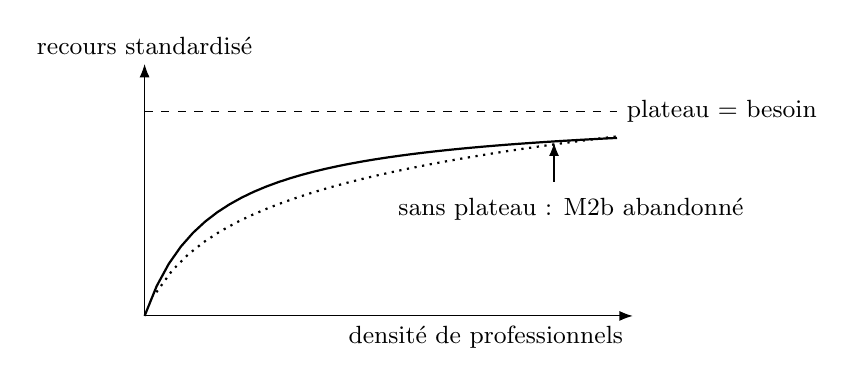
\begin{tikzpicture}[x=1cm,y=1cm]
  \draw[-{Latex}] (0,0) -- (6.2,0) node[below left] {\small densité de professionnels};
  \draw[-{Latex}] (0,0) -- (0,3.2) node[above] {\small recours standardisé};
  \draw[thick,domain=0:6,samples=40] plot (\x,{2.6*\x/(\x+0.9)});
  \draw[dashed] (0,2.6) -- (6,2.6) node[right] {\small plateau = besoin};
  \draw[thick,dotted,domain=0.15:6,samples=30] plot (\x,{0.9+0.75*ln(\x+0.3)});
  \node[anchor=west] at (3.1,1.35) {\small sans plateau : M2b abandonné};
  \draw[{Latex}-] (5.2,2.2) -- (5.2,1.7);
\end{tikzpicture}
\caption{Ce que teste P-B2 (formes \emph{schématiques}). Courbe pleine : saturation, M2b vit. Courbe pointillée :
croissance sans plafond, M2b est abandonné.}
\end{figure}

\subsection*{M3 : épidémiologique}
\[
B_3 \;=\; \sum_{\text{maladies}} \text{population} \times \text{prévalence de la maladie} \times
\text{actes nécessaires par patient}.
\]
Les prévalences viennent de la cartographie des pathologies de l'Assurance maladie : par département, âge et sexe,
pour 61\mesure{} groupes de maladies, de 2015 à 2024\mesure{}. Pour les sages-femmes, le besoin se construit à partir
des naissances et du nombre d'examens par grossesse.

C'est \textbf{le seul estimateur qui ne dépend pas de l'offre}. Il voit aussi la morbidité locale, pas seulement l'âge.
C'est le cadre classique de la planification des effectifs fondée sur le besoin \citep{birch2007,mackenzie2019}. Sa
limite est le nombre d'\enquote{actes nécessaires par patient} : il vient soit d'une norme (une recommandation), soit
du recours national, qui est lui-même contraint.

\subsection*{M4 : l'accès dans l'espace}
On se soigne souvent dans la commune d'à côté. M4 calcule, pour chaque commune, l'offre accessible depuis elle :
celle des communes voisines, pondérée par le temps de trajet, rapportée à la population qui s'y adresse aussi. C'est
la famille de méthodes appelée 2SFCA \citep{luo2009}, celle de l'indicateur APL de la DREES \citep{barlet2012}.

\begin{figure}[h]
\centering
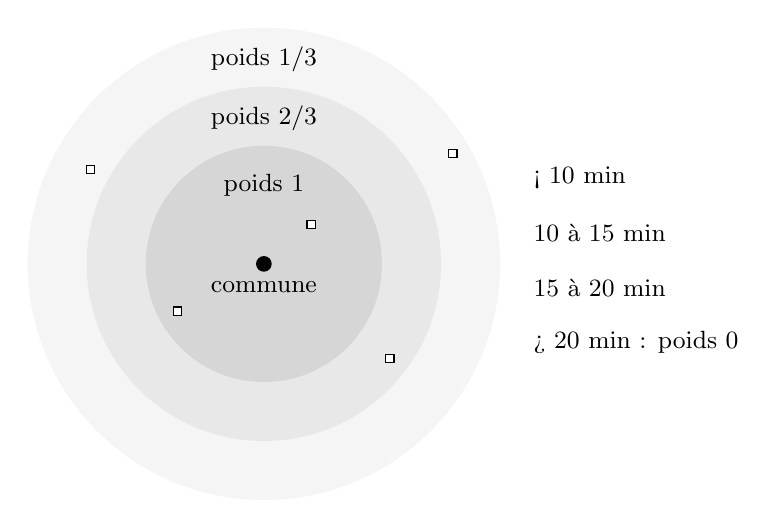
\begin{tikzpicture}
  \fill[gray!8] (0,0) circle (3);
  \fill[gray!18] (0,0) circle (2.25);
  \fill[gray!32] (0,0) circle (1.5);
  \node[circle,fill=black,inner sep=2pt,label=below:{\small commune}] at (0,0) {};
  \node at (0,1.0) {\small poids 1};
  \node at (0,1.85) {\small poids 2/3};
  \node at (0,2.6) {\small poids 1/3};
  \node[anchor=west,align=left] at (3.3,1.1) {\small < 10 min};
  \node[anchor=west,align=left] at (3.3,0.4) {\small 10 à 15 min};
  \node[anchor=west,align=left] at (3.3,-0.3) {\small 15 à 20 min};
  \node[anchor=west,align=left] at (3.3,-1.0) {\small > 20 min : poids 0};
  \foreach \p in {(0.6,0.5),(-1.1,-0.6),(1.6,-1.2),(-2.2,1.2),(2.4,1.4)} \node[draw,fill=white,inner sep=1.5pt] at \p {};
\end{tikzpicture}
\caption{Pondération par le temps de trajet pour les infirmiers, kinés et dentistes (paramètres publiés par la DREES ;
pour les sages-femmes, les paliers vont jusqu'à 30~min). Les carrés représentent des professionnels.}
\end{figure}

M4 ne définit pas le besoin. Il prend celui de M1, M2 ou M3 et le croise avec l'offre et la distance. Il apporte deux
choses :
\begin{itemize}
  \item il franchit les frontières administratives et descend à la commune ;
  \item projeté jusqu'en 2050 avec des poids d'âge \emph{figés} à une année de base, il voit le vieillissement
    national. La DREES recalcule ses poids à chaque millésime, si bien que son APL ne peut pas comparer deux années
    sous l'effet du vieillissement.
\end{itemize}
Ses limites : il n'existe pas d'APL des pharmaciens, et l'activité individuelle de chaque professionnel, que la DREES
utilise, n'est pas publique.

\section{Les transferts de tâches}
Un transfert fait passer un acte d'une profession A, par exemple les médecins généralistes, à une profession B,
par exemple les pharmaciens. Le jumeau ne crée ni ne supprime aucun professionnel : seul le besoin se déplace.
\[
B'_A = B_A\,(1 - s\,a), \qquad
B'_B = B_B + s\,a\,k\,B_A + m .
\]
\begin{itemize}
  \item $a$ : la part du temps de A consacrée à cet acte ;
  \item $s(t)$ : la part effectivement transférée. Elle monte progressivement après l'autorisation, comme une
    innovation qui se diffuse ;
  \item $k$ : la durée de l'acte chez B rapportée à sa durée chez A ($k<1$ : B est plus rapide) ;
  \item $m$ : les nouveaux patients, qui n'auraient pas eu l'acte du tout sans le transfert.
\end{itemize}
Le besoin total change exactement de $s\,a\,B_A\,(k-1)+m$. C'est une identité que le code vérifie automatiquement.

\paragraph{L'exemple de la vaccination antigrippale en officine.}
C'est le seul transfert pour lequel les données ouvertes permettent d'estimer $a$ et $s(t)$.
\begin{itemize}
  \item \textbf{La part des pharmaciens a doublé.} Ils assuraient un peu moins d'une vaccination antigrippale sur
    trois en 2019-20, et près de deux sur trois en 2024-25\mesure{}. Sur la même période, la part des médecins est
    passée d'une sur deux à moins d'une sur quatre \citep{ccomptes2026}.
  \item \textbf{Les volumes en officine continuent de monter} : \num{5645127} actes en 2023-24, \num{6629119} en
    2024-25, puis \num{8020525} en 2025-26, au 28 février\mesure{}. Ces chiffres sont extrapolés d'un panel d'environ
    60~\% des officines (IQVIA, data.gouv.fr).
  \item \textbf{La diffusion suit la date d'entrée des régions.} L'expérimentation a commencé en octobre 2017 en
    Auvergne-Rhône-Alpes et en Nouvelle-Aquitaine, puis en octobre 2018 dans les Hauts-de-France et en Occitanie,
    avant d'être généralisée en 2019-20. En 2019-20, la part des pharmaciens atteignait 36,7~\%\mesure{} dans les
    régions de 2017, contre 25,6~\%\mesure{} dans celles de 2019 \citep{liard2022}. C'est une observation directe de
    $s(t)$.
  \item \textbf{$m$ semble faible.} Au Canada, la mesure a augmenté la couverture d'environ 5~\%\mesure{} en valeur
    relative \citep{buchan2017}. En France, la première année, la couverture valait 46,1~\%\mesure{} dans les
    régions de l'expérimentation, contre 46,0~\% la saison précédente.
  \item \textbf{$k$ n'est pas mesuré} : aucune source ne donne la durée d'une vaccination en officine. Il reste
    \enquote{supposé}. Quand un infirmier remplace un médecin, les consultations sont plutôt plus longues, donc
    $k>1$ \citep{laurant2018}.
\end{itemize}

\paragraph{La médecine générale.} Elle est exclue du sujet. Or la plupart des transferts annoncés lui prennent des
actes. Décision de l'équipe (option O2) : la médecine générale apparaît \emph{seulement comme source}. On affiche
\enquote{$x$ actes de médecine générale libérés}, jamais un indice de couverture pour elle.

\paragraph{La réponse honnête à la question du sujet.} \enquote{À Clermont-Ferrand en 2035, si les pharmaciens
vaccinent, l'effectif ne change pas dans le modèle. La couverture des pharmaciens baisse de $y$~\%, et le modèle
indique combien d'actes de médecine générale sont libérés.}

\section{Comment on décide : des tests écrits avant les calculs}
Pour ne pas choisir l'estimateur qui \enquote{donne le résultat qu'on aime}, chaque test est rédigé avec son critère
d'abandon \emph{avant} de voir les données, puis gelé.

\begin{table}[h]
\centering\small
\begin{tabularx}{\linewidth}{@{}l X X@{}}
\toprule
\textbf{Test} & \textbf{Question} & \textbf{Ce qui fait abandonner} \\
\midrule
P-B1 & L'âge change-t-il l'indice en 2050 (M1 contre M0) ? & écart < 2~\%\suppose{} dans plus de 90~\%\suppose{} des départements, classement inchangé \\
P-B2 & Le recours plafonne-t-il quand l'offre augmente ? & pas de plateau : M2b abandonné \\
P-B3 & Les maladies apportent-elles quelque chose au-delà de l'âge (M3 contre M1) ? & même règle que P-B1 \\
P-B4 & Sait-on reproduire l'APL 2024 de la DREES ? & corrélation de rang < 0,90\suppose{}, ou pas mieux que la densité simple \\
P-B5 & L'âge prédit-il l'évolution du recours entre 2016 et 2025 ? & pas mieux que \enquote{recours par habitant constant} pour au moins 3 professions sur 5 \\
P-B6 & La vaccination en officine a-t-elle ajouté des vaccinations ($m$) ? & effet nul sur le total des doses \\
\bottomrule
\end{tabularx}
\caption{Les six protocoles pré-enregistrés. Les seuils sont des choix (\suppose), fixés avant le calcul.}
\end{table}

L'historique git ne prouve pas qu'un protocole a été écrit avant le calcul. L'empreinte numérique des protocoles a donc
été déposée auprès de deux services d'horodatage indépendants (FreeTSA et DigiCert), qui en certifient la date.
Seule l'empreinte, et non le texte, a été envoyée.

Un modèle d'apprentissage automatique ne sert pas à estimer le besoin : le besoin n'est jamais observé, il n'y a donc
pas de \enquote{bonne réponse} sur laquelle apprendre. Un tel modèle ne peut entrer qu'en concurrent dans le backtest
P-B5, s'il y bat M1.

\section{Les données}
\begin{table}[h]
\centering\small
\begin{tabularx}{\linewidth}{@{}l X l l@{}}
\toprule
\textbf{Jeu} & \textbf{Ce qu'il donne} & \textbf{Grain} & \textbf{Sert à} \\
\midrule
Open DAMIR & actes remboursés par profession, âge, sexe ; mensuel, 2009--2025 & région (13 zones) & M1, P-B6 \\
Patientèle (ameli) & patients uniques par profession, 2016--2025, sans les pharmaciens & département & P-B2, P-B5 \\
Pathologies (ameli) & prévalence de 61 groupes de maladies, 2015--2024 & département & M3 \\
APL (DREES) & accessibilité 2022--2024, poids d'âge, paliers & commune & M1, M4, P-B4 \\
Omphale (Insee) & population projetée par âge jusqu'en 2070 & département & tous \\
IQVIA, Cour des comptes & vaccination en officine & national, région & transferts \\
\bottomrule
\end{tabularx}
\caption{Sources ouvertes. Aucune ne donne d'actes par profession au département : c'est la principale contrainte.}
\end{table}

\section{Ce que le module ne fait pas}
\begin{itemize}
  \item Il ne fait pas réagir les effectifs au besoin. Un test du projet a mesuré un effet nul de la densité sur les
    installations : le jumeau ne suppose donc pas que les professionnels s'installent là où le besoin est fort.
  \item Il ne dit pas quel est le \enquote{bon} niveau de soins. L'indice compare un territoire à lui-même en 2026.
  \item Il ne modélise ni les prix, ni le reste à charge, ni la dérive des habitudes de consommation par âge.
  \item Sur 25 paramètres de transfert et de besoin, 14 sont aujourd'hui non mesurables à partir de données ouvertes.
    Les transferts autres que la vaccination restent donc \enquote{supposés} ou \enquote{hors modèle}.
\end{itemize}

\section{Où on en est (15 novembre 2026)}
\begin{itemize}
  \item \textbf{Fait :}
    \begin{itemize}
      \item l'interface de code, M0 et l'opérateur de transfert, qui passent 7 tests d'identité sur 7 ;
      \item les fiches de paramètres ;
      \item les six protocoles, gelés et horodatés ;
      \item l'ingestion des données ameli, de l'APL et de la vaccination.
    \end{itemize}
  \item \textbf{En cours :} l'agrégation d'Open DAMIR, lue en flux sans stocker les fichiers bruts.
  \item \textbf{Ensuite :}
    \begin{itemize}
      \item M1 à M4 et les transferts ;
      \item les six tests, en commençant par P-B1, le moins cher, qui peut à lui seul simplifier le module ;
      \item une analyse de sensibilité : le choix de l'estimateur pèse-t-il plus que la politique simulée ?
    \end{itemize}
\end{itemize}

\section*{Glossaire}
\begin{description}[leftmargin=2.2cm,style=nextline]
  \item[Besoin] soins nécessaires compte tenu de l'état de santé, qu'ils soient obtenus ou non. Non observé.
  \item[Recours] soins réellement consommés (actes remboursés). Observé.
  \item[Demande induite] activité supplémentaire générée par l'abondance de l'offre.
  \item[Indice $C$] offre rapportée au besoin, comparée à 2026 ; $C<1$ = couverture moindre qu'aujourd'hui.
  \item[APL] accessibilité potentielle localisée, l'indicateur communal d'accès aux soins de la DREES.
  \item[2SFCA] méthode de calcul de l'accès en deux étapes, offre puis population, avec pondération par la distance.
  \item[Pré-enregistrement] écrire un test et son critère d'échec avant de voir le résultat.
  \item[Omphale] le modèle de projection de la population de l'Insee.
\end{description}

\bibliographystyle{plainnat}
\bibliography{refs}
\end{document}
